\documentclass[glossy]{beamer}
\useoutertheme{wuerzburg}
\useinnertheme[realshadow,corners=2pt,padding=2pt]{chamfered}
\usecolortheme{shark}

\usepackage{listings}
\usepackage[utf8]{inputenc}


\usepackage{fancyvrb}
%\usepackage[scaled]{beramono} %sets the beramono font. Just comment this line to get the default font back

\usepackage{tikz}
\newcommand<>{\hover}[1]{\uncover#2{%
 \begin{tikzpicture}[remember picture,overlay]%
 \draw[fill,opacity=0.4] (current page.south west)
 rectangle (current page.north east);
 \node at (current page.center) {#1};
 \end{tikzpicture}}
}

\title{Arquitecturas y Organización de Computadoras I \\\line(1,0){320}}
% \author{\texorpdfstring{Author\newline\url{email@email.com}}{Author}}
%\author{Rafael Ignacio Zurita}
\institute{Rafael Ignacio Zurita \\ Departamento de Ingenieria de Computadoras - FAI - UNCOMA 2018 \\ Clase presencial 7}
%\date{\today}



\begin{document}




\begin{frame}
\maketitle
\end{frame}

\institute{Departamento de Ingenieria de Computadoras - FAI - UNCOMA \\ 2018}

\begin{frame}
\frametitle{Programa Analítico}
\textbf{UNIDAD 2: Unidad Central de Proceso}
 \\~\\
Introducción al diseño lógico. Tablas de verdad. Álgebra de Boole.  Circuitos  combinacionales.  Relojes.  Elementos  de memoria.  Flip-flops,  cerrojos (latches) .  Circuitos  secuenciales.  Implementación de FSM. Circuitos lógicos programables. Unidad Lógica aritmética. Implementación de la suma, resta y operaciones lógicas.  Concepto  de  máquinas  algorítmicas.  \textbf{Camino  de  datos.  Unidad  de  control.}  Implementación  del  algoritmo    básico  de multiplicación. Conceptos de representación de número en punto flotante y error. Suma y multiplicación de punto flotante.
 \\~\\
\end{frame}


\begin{frame}
\frametitle{Temario}
\begin{itemize}
\item Circuitos combinacionales y secuenciales necesarios
\item Camino de datos de un sólo ciclo
\item Camino de datos multiciclo
\item Camino de datos segmentado
\end{itemize}
\end{frame}




\begin{frame}
\frametitle{Temario}
        \begin{center}
        \textbf{Cuando se quiere comprar una computadora nueva...}
        \end{center}
\begin{tabular}{cl}

\begin{tabular}{c}
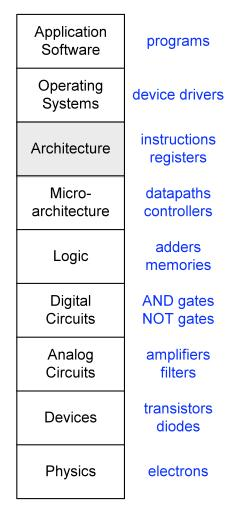
\includegraphics[height=6cm, width=4cm]{estructura-por-niveles.jpg} 

\end{tabular}
& \begin{tabular}{l}
\parbox{0.5\linewidth}{
        \textbf{Microarquitectura} \\
        Como implementar una arquitectura en hardware (meta: costo, rendimiento, etc) \\
        La microarquitectura es construída por circuitos lógicos y elementos de memoria \\
        Todos los circuitos lógicos y elementos de memoria son implementados físicamente con transistores
}
\end{tabular} \\

\end{tabular}
\end{frame}





\begin{frame}
\frametitle{Implementación de la Microarquitectura}
\begin{center}\textbf{Diseño de la Microarquitectura (diseño del procesador)}\end{center}
\begin{enumerate}
\item Analizar el conjunto de instrucciones (ISA)
\begin{itemize}
\item Obtener los requerimientos del camino de datos
\end{itemize}
\item Seleccionar los \textit{componentes} y establecer la \textit{metodología} del reloj
\item Componer el \textit{camino de datos} para cumplir los requerimientos
\item Determinar las \textit{señales de control} para cada instrucción
\item Componer la \textit{lógica de control (unidad de control)} para generar las señales de control
\end{enumerate}
\end{frame}



\begin{frame}
\frametitle{Implementación de la Microarquitectura}
\begin{center}\textbf{Diseño de la Microarquitectura (diseño del procesador)}\end{center}
\begin{enumerate}
\item Analizar el conjunto de instrucciones (ISA)
\begin{itemize}
\item \textbf{Obtener los requerimientos del camino de datos}
\end{itemize}
\item Seleccionar los \textit{componentes} y establecer la \textit{metodología} del reloj
\item Componer el \textit{camino de datos} para cumplir los requerimientos
\item Determinar las \textit{señales de control} para cada instrucción
\item Componer la \textit{lógica de control (unidad de control)} para generar las señales de control
\end{enumerate}
\end{frame}


\begin{frame}
\frametitle{Implementación de la Microarquitectura}
\begin{center}\textbf{Diseño de la Microarquitectura (diseño del procesador)}\end{center}
\begin{figure}
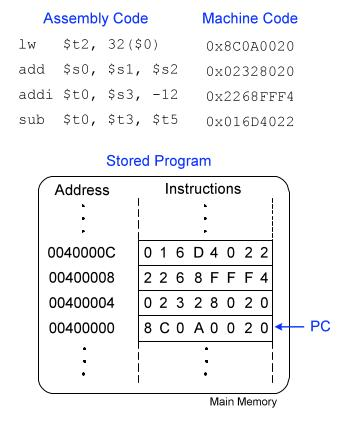
\includegraphics[scale=0.2]{programa-almacenado.jpg} 
\end{figure}
\begin{figure}
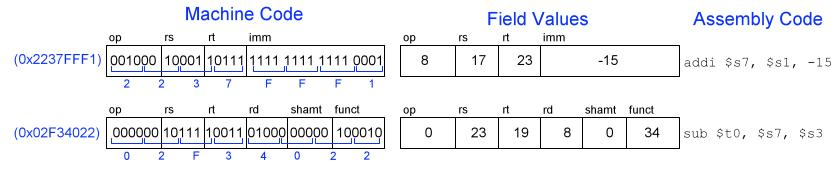
\includegraphics[scale=0.2]{codigo-maquina.jpg} 
\end{figure}
\end{frame}

%\begin{frame}
%\frametitle{Implementación de la Microarquitectura}
%\begin{center}\textbf{Analizar el conjunto de instrucciones (ISA) \end{center}
%\begin{figure}
%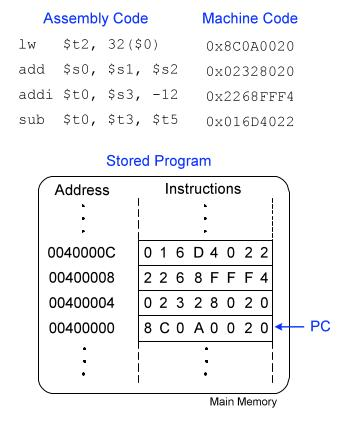
\includegraphics[scale=0.4]{programa-almacenado.jpg} 
%\end{figure}
%
%\begin{figure}
%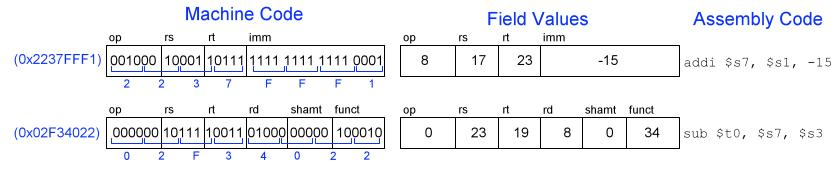
\includegraphics[scale=0.4]{codigo-maquina.jpg} 
%\end{figure}
%
%\end{frame}





\begin{frame}
\frametitle{Implementación de la Microarquitectura}
\begin{center}\textbf{Diseño de la Microarquitectura (diseño del procesador)}\end{center}
\begin{enumerate}
\item Analizar el conjunto de instrucciones (ISA)
\begin{itemize}
\item Obtener los requerimientos del camino de datos
\end{itemize}
\item \textbf{Seleccionar los \textit{componentes} y establecer la \textit{metodología} del reloj}
\item Componer el \textit{camino de datos} para cumplir los requerimientos
\item Determinar las \textit{señales de control} para cada instrucción
\item Componer la \textit{lógica de control (unidad de control)} para generar las señales de control
\end{enumerate}
\end{frame}



\begin{frame}
\frametitle{Implementación de la Microarquitectura}
\begin{center}\textbf{Diseño de la Microarquitectura (diseño del procesador)}\end{center}
\begin{enumerate}
\item Analizar el conjunto de instrucciones (ISA)
\begin{itemize}
\item Obtener los requerimientos del camino de datos
\end{itemize}
\item Seleccionar los \textit{componentes} y establecer la \textit{metodología} del reloj
\item \textbf{Componer el \textit{camino de datos} para cumplir los requerimientos}
\item Determinar las \textit{señales de control} para cada instrucción
\item Componer la \textit{lógica de control (unidad de control)} para generar las señales de control
\end{enumerate}
\end{frame}








\begin{frame}
\frametitle{Compuertas, Tablas de Verdad, Ecuaciones Lógicas}
\begin{center}\textbf{Señales digitales}\end{center}
\begin{itemize}
\item Esta es una razón clave por la que los 
computadores utilizan números binarios, ya 
que un sistema binario se corresponde 
directamente con la abstracción subyacente a 
la electrónica
\item En las diferentes implementaciones 
electrónicas los voltajes y sus relaciones difieren,
\item Por lo que no se utiliza el valor del voltage sino una indicación de si la señal esta activada o no (verdadera o no, 1 o 0, etc).

\end{itemize}
\end{frame}





\begin{frame}
\frametitle{Compuertas, Tablas de Verdad, Ecuaciones Lógicas}
\begin{center}\textbf{Señales digitales}\end{center}
\begin{itemize}
\item Por eso hablamos de señales que son:
\begin{itemize}
\item (lógicamente) ciertas, ó 1, ó 
afirmadas, asertadas
\item (lógicamente) falsas, ó 0, ó  
negadas
\end{itemize}
\item Los valores 0 y 1 reciben el nombre de 
complementarios o inversos
 el uno del otro

\end{itemize}
\end{frame}



\begin{frame}
\frametitle{Compuertas, Tablas de Verdad, Ecuaciones Lógicas}
\begin{center}\textbf{Diseño digital}\end{center}
\begin{itemize}
\item Los bloques lógicos 
(circuitos digitales o lógicos)
 se 
clasifican en dos tipos:
\begin{itemize}
\item circuitos combinacionales
\begin{itemize}
\item Sus salidas dependen sólo de las entradas
\end{itemize}
\item circuitos secuenciales

\begin{itemize}
\item Mantienen un estado interno. Sus salidas pueden 
depender tanto de las entradas actuales como
del valor almacenado en memoria, conocido 
como estado del bloque
\end{itemize}

\end{itemize}
\end{itemize}
\end{frame}





\begin{frame}
\frametitle{Compuertas, Tablas de Verdad, Ecuaciones Lógicas}
\begin{center}\textbf{Tablas de Verdad}\end{center}
\begin{itemize}
\item Debido a que un bloque de lógica combinatoria 
no contiene memoria, puede especificarse 
completamente definiendo los valores de las 
salidas para cada posible conjunto de valores 
de entrada
\item 
Dicha descripción se da normalmente en forma 
de 
tabla de verdad

\end{itemize}
\end{frame}




\begin{frame}
\frametitle{Compuertas, Tablas de Verdad, Ecuaciones Lógicas}
\begin{center}\textbf{Tablas de Verdad}\end{center}
\begin{itemize}
\item Para un bloque lógico con n entradas, existen   2 n posiciones en la tabla de verdad, puesto que 
este es el número de combinaciones posible de 
los valores de entrada
\item Cada posición en la tabla especifica el valor de 
todas las salidas para una combinación 
particular de las entrada
\item Las tablas de verdad pueden \textbf{describir 
completamente cualquier función lógica} 
combinatoria
\item Sin embargo, su tamaño \textbf{crece rápidamente} y 
puede dificultar su comprensión

\end{itemize}
\end{frame}


%\begin{frame}
%\frametitle{Compuertas, Tablas de Verdad, Ecuaciones Lógicas}
%\begin{center}\textbf{Tablas de Verdad}\end{center}
%\begin{figure}
%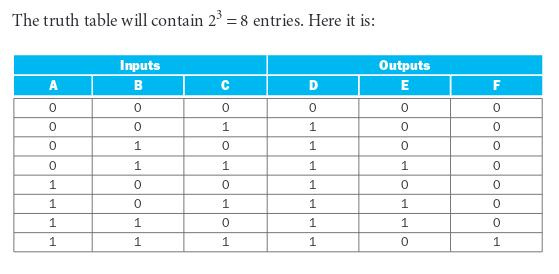
\includegraphics[scale=0.4]{tabla.jpg} 
%\end{figure}
%
%
%\end{frame}











\begin{frame}
\frametitle{Compuertas, Tablas de Verdad, Ecuaciones Lógicas}
\begin{center}\textbf{Algebra de Boole}\end{center}
\begin{itemize}
\item Todas la variable tienen valores 0 ó 1
\item Existen tres operadores:
\begin{itemize}
\item \textbf{OR}
, se escribe 
+
, como en 
A +B
. El resultado es 1 si alguna 
de la variables de entrada es 1. También se conoce como 
suma lógica
\item \textbf{AND}
, se escribe
 .
, como en
 A.B
. El resultado es 1 sólo si 
ambas entradas son 1. También se conoce como 
producto 
lógico
\item \textbf{NOT}
, se escribe      . El resultado es 1 sólo si la entrada es 0. 
La aplicación del operador NOT a un valor lógico resulta en 
una inversión o negación de dicho valor 
\end{itemize}
\end{itemize}
\end{frame}






\begin{frame}
\frametitle{Compuertas, Tablas de Verdad, Ecuaciones Lógicas}
\begin{center}\textbf{Álgebra de Boole - Leyes y Teoremas}\end{center}
\begin{figure}
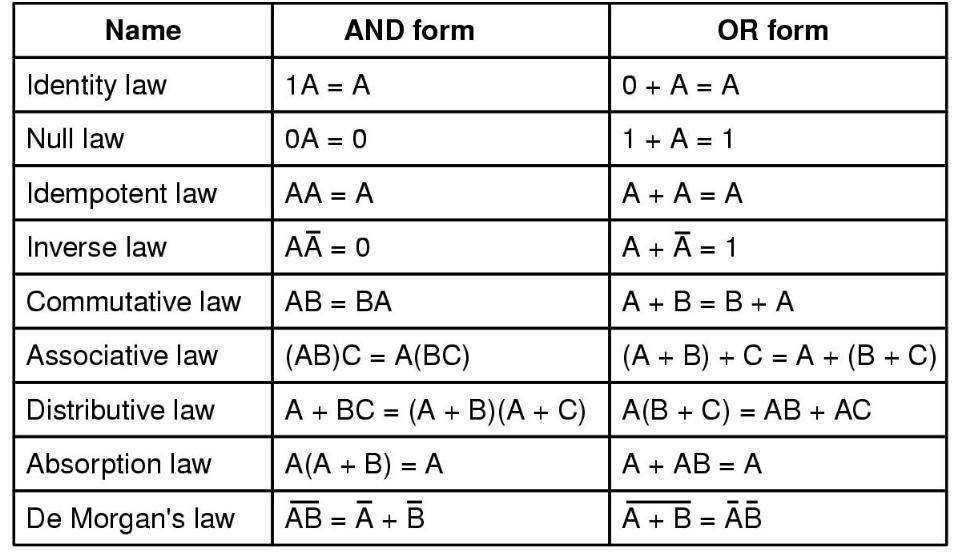
\includegraphics[scale=0.2]{leyes.jpg} 
\end{figure}
\end{frame}







\begin{frame}
\frametitle{Compuertas, Tablas de Verdad, Ecuaciones Lógicas}
\begin{center}\textbf{Álgebra de Boole - Leyes y Teoremas}\end{center}
\begin{itemize}
\item Cualquier función lógica puede ser reescrita como una ecuación, 
con la salida en la parte izquierda de la igualdad, y una función 
de las variables de entrada utilizando las operaciones del álgebra a la derecha.

\item Ejemplo:
\end{itemize}
\begin{figure}
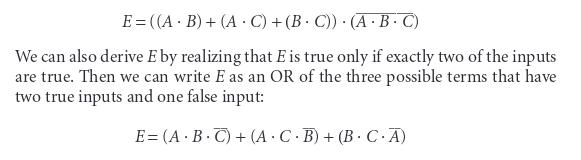
\includegraphics[scale=0.4]{ecuacion.jpg} 
\end{figure}
\end{frame}




\begin{frame}[fragile]
\frametitle{Diseño digital}
\begin{center}\textbf{Compuertas/Puertas (Gates)}\end{center}
\begin{itemize}
\item Los bloques lógicos se construyen a partir de 
compuertas (puertas) lógicas
 que realizan las 
funciones lógicas básicas como AND, OR y NOT
\item Una puerta AND o una OR pueden tener 
múltiples entradas, con la salida igual a la AND o 
la OR de todas ellas
\item La función lógica NOT se realiza mediante un 
inversor que siempre tiene una entrada
\end{itemize}

\end{frame}





\begin{frame}[fragile]
\frametitle{Diseño digital}
\begin{center}\textbf{Compuertas/Puertas (Gates)}\end{center}
\begin{figure}
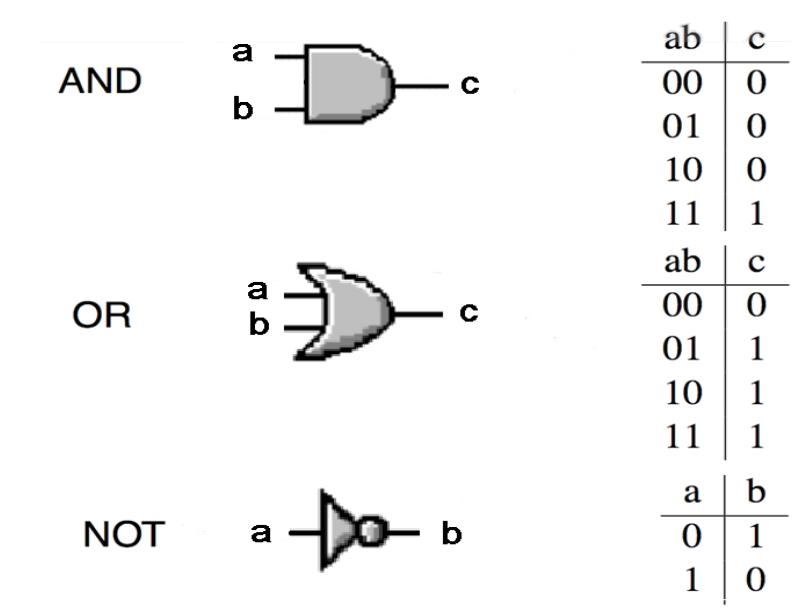
\includegraphics[scale=0.2]{compuertas.jpg} 
\end{figure}
\end{frame}


\begin{frame}[fragile]
\frametitle{Diseño digital}
\begin{center}\textbf{Compuertas/Puertas (Gates)}\end{center}
\begin{figure}
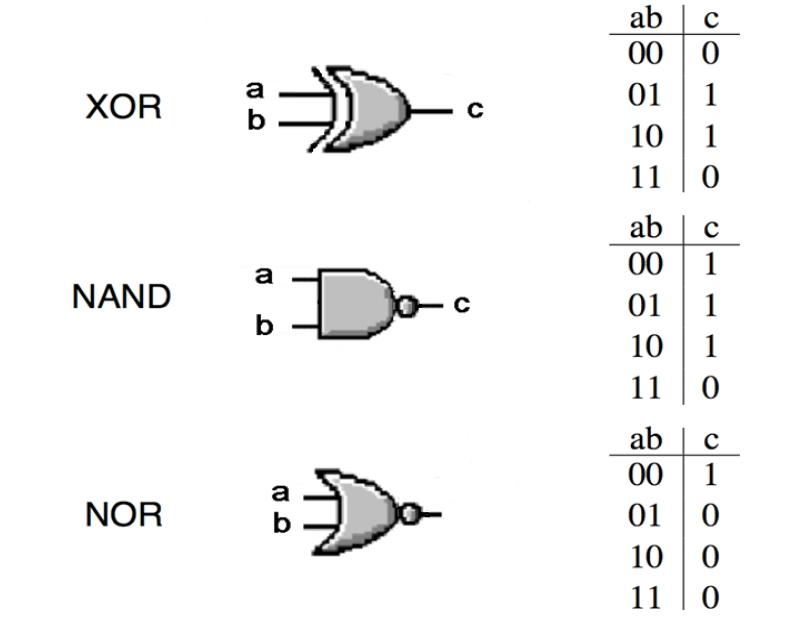
\includegraphics[scale=0.2]{compuertasx.jpg} 
\end{figure}
\end{frame}


\begin{frame}[fragile]
\frametitle{Diseño digital}
\begin{center}\textbf{Construcción de diseño lógico/digital}\end{center}
\begin{figure}
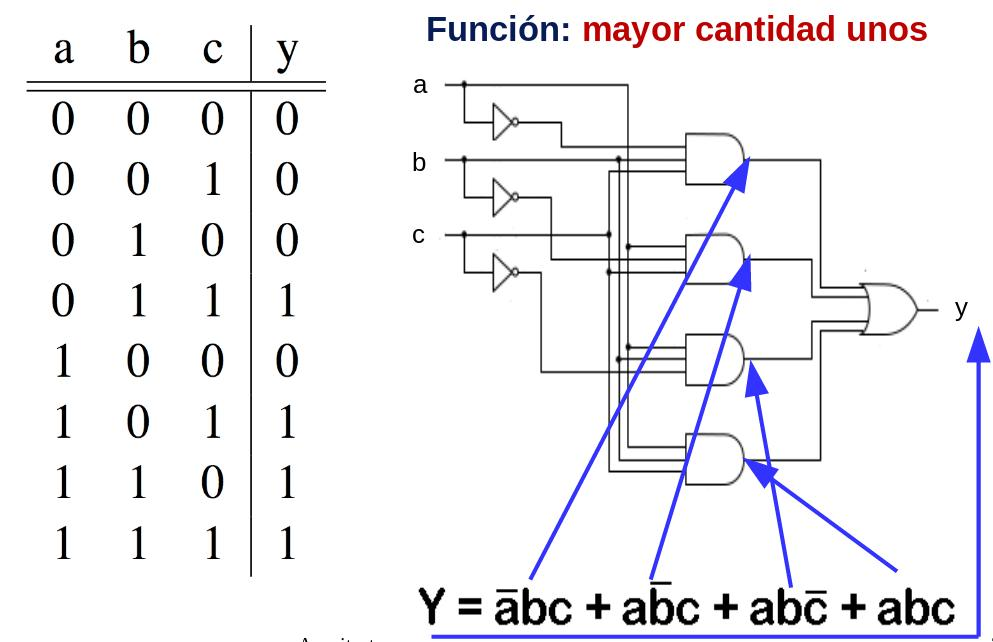
\includegraphics[scale=0.2]{construcciondigital.jpg} 
\end{figure}
\end{frame}




\begin{frame}[fragile]
\frametitle{Diseño digital}
\begin{center}\textbf{Construcción de diseño lógico/digital: Decoder}\end{center}
\begin{figure}
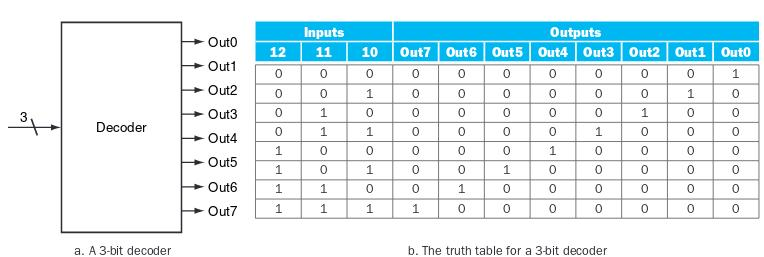
\includegraphics[scale=0.4]{decoder.jpg} 
\end{figure}
\end{frame}


\begin{frame}[fragile]
\frametitle{Diseño digital}
\begin{center}\textbf{Construcción de diseño lógico/digital: Multiplexor}\end{center}
\begin{figure}
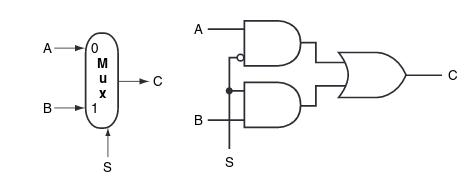
\includegraphics[scale=0.4]{multiplexor.jpg} 
\end{figure}
\end{frame}



\begin{frame}[fragile]
\frametitle{Diseño digital}
\begin{center}\textbf{Construcción de diseño lógico/digital: Multiplexor 32 bits}\end{center}
\begin{figure}
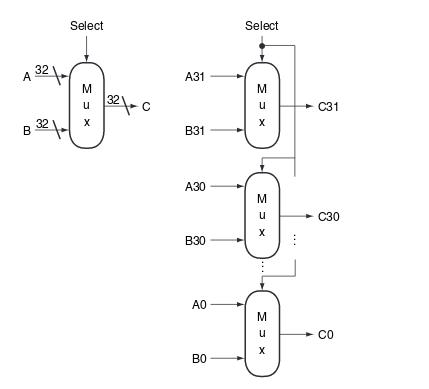
\includegraphics[scale=0.4]{multiplexor32bits.jpg} 
\end{figure}
\end{frame}




\begin{frame}[fragile]
\frametitle{Diseño digital}
\begin{center}\textbf{Diseño de ALU de un bit}\end{center}
\begin{figure}
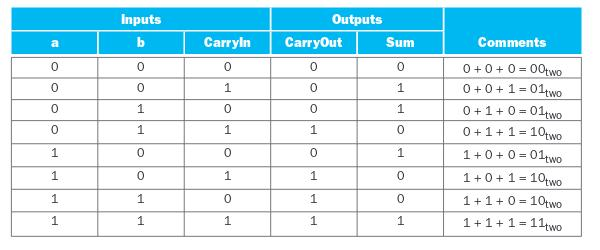
\includegraphics[scale=0.4]{alu1bit.jpg} 
\end{figure}
\end{frame}




\begin{frame}[fragile]
\frametitle{Diseño digital}
\begin{center}\textbf{Diseño de ALU de un bit}\end{center}
\begin{figure}
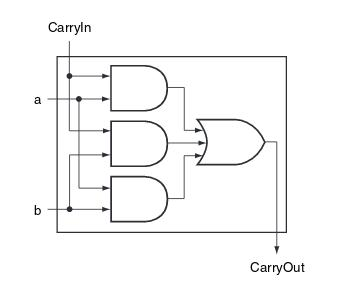
\includegraphics[scale=0.4]{alu1bit-2.jpg} 
\end{figure}
\end{frame}




\begin{frame}[fragile]
\frametitle{Diseño digital}
\begin{center}\textbf{Diseño de ALU de un bit}\end{center}
\begin{figure}
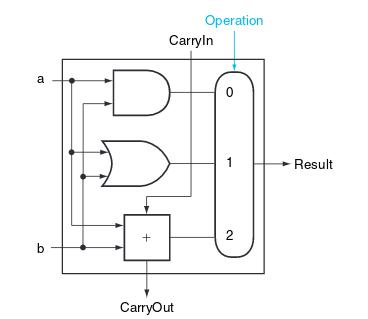
\includegraphics[scale=0.4]{alu1bit-3.jpg} 
\end{figure}
\end{frame}


\begin{frame}[fragile]
\frametitle{Diseño digital}
\begin{center}\textbf{Diseño de ALU de un bit}\end{center}
\begin{figure}
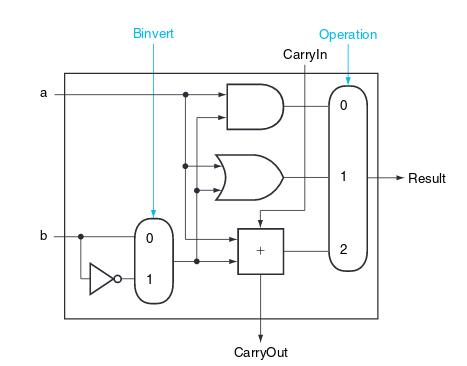
\includegraphics[scale=0.4]{alu1bit-4.jpg} 
\end{figure}
\end{frame}


\begin{frame}[fragile]
\frametitle{Diseño digital}
\begin{center}\textbf{Diseño de ALU de 32 bits}\end{center}
\begin{figure}
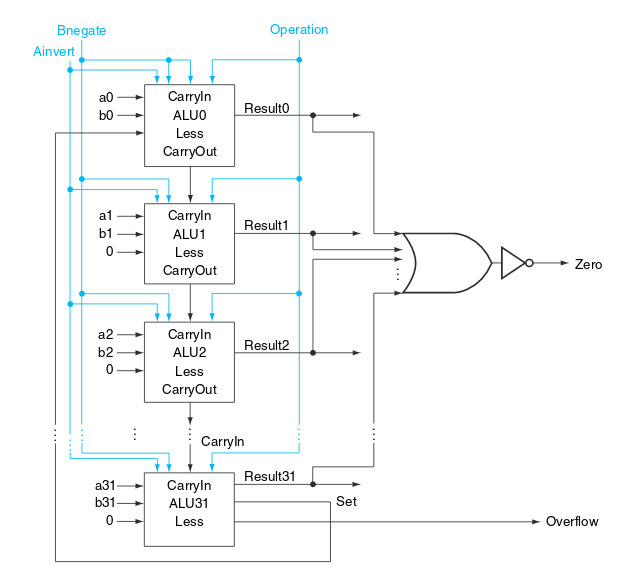
\includegraphics[scale=0.4]{alu1bit-5.jpg} 
\end{figure}
\end{frame}


\begin{frame}[fragile]
\frametitle{Diseño digital}
\begin{center}\textbf{Diseño de una unidad de control}\end{center}
\begin{figure}
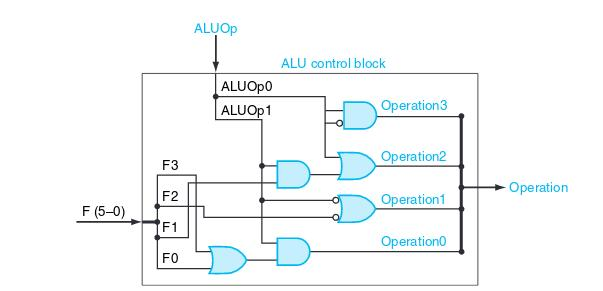
\includegraphics[scale=0.4]{control.jpg} 
\end{figure}
\end{frame}


\begin{frame}[fragile]
\frametitle{Diseño digital}
\begin{center}\textbf{Relojes}\end{center}
\begin{itemize}
\item Los relojes son necesarios en la lógica secuencial, para decidir cuando un elemento que contiene un estado debe ser actualizado.
\item Terminología: tiempo del ciclo (período), frecuencia del reloj.
\item Metodología : edge-triggered clocking (reloj disparado por flanco)
\end{itemize}
\begin{figure}
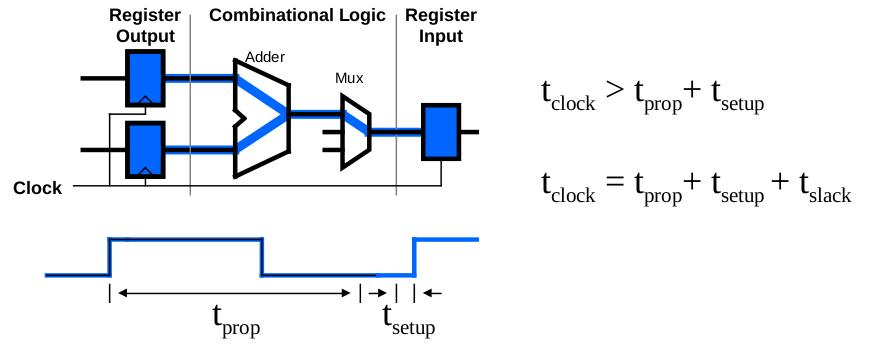
\includegraphics[scale=0.4]{reloj.jpg} 
\end{figure}
\end{frame}


\begin{frame}[fragile]
\frametitle{Diseño digital}
\begin{center}\textbf{Relojes}\end{center}
\begin{itemize}
\item Sistemas síncronos
\item edge-triggered clocking posibilita un proceso instantáneo
\end{itemize}
\begin{figure}
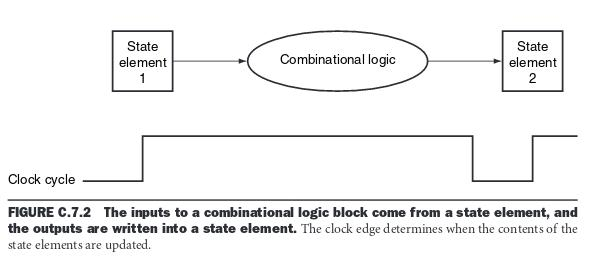
\includegraphics[scale=0.4]{reloj-estado-combinacional.jpg} 
\end{figure}
\end{frame}


\begin{frame}[fragile]
\frametitle{Diseño digital}
\begin{center}\textbf{Elementos de memoria (circuitos secuenciales)}\end{center}
\begin{itemize}
\item Set-Reset Latch
\item Elemento básico para almacenar un bit. Contiene un Loop en su diseño.
\end{itemize}
\begin{figure}
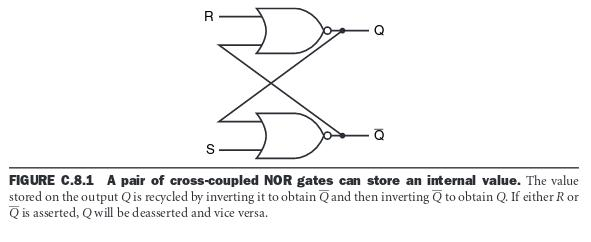
\includegraphics[scale=0.4]{latch-s-r.jpg} 
\end{figure}
\end{frame}

\begin{frame}[fragile]
\frametitle{Diseño digital}
\begin{center}\textbf{Elementos de memoria (circuitos secuenciales)}\end{center}
\begin{itemize}
\item D-Latch
\item Elemento básico para almacenar un bit. Contiene un Loop en su diseño
\item Sus entradas son el bit a almacenar y la señal de reloj
\end{itemize}
\begin{figure}
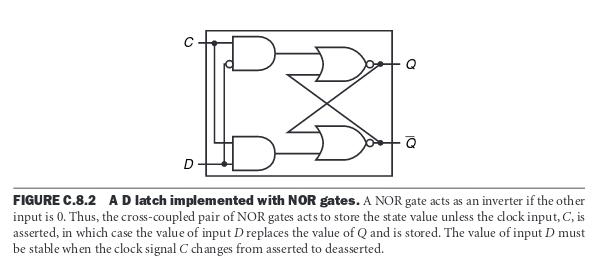
\includegraphics[scale=0.4]{latch-d.jpg} 
\end{figure}
\end{frame}


\begin{frame}[fragile]
\frametitle{Diseño digital}
\begin{center}\textbf{Elementos de memoria (circuitos secuenciales)}\end{center}
\begin{itemize}
\item D-Latch
\end{itemize}
\begin{figure}
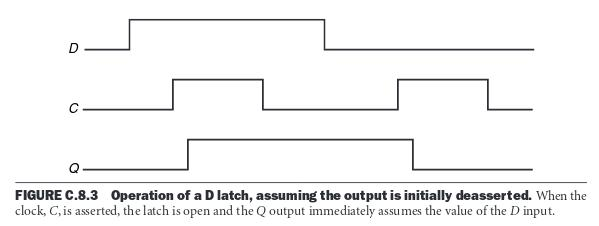
\includegraphics[scale=0.4]{latch-d-tiempo.jpg} 
\end{figure}
\end{frame}


\begin{frame}[fragile]
\frametitle{Diseño digital}
\begin{center}\textbf{Elementos de memoria (circuitos secuenciales)}\end{center}
\begin{itemize}
\item D Flip-Flop : utilizados en la construcción de REGISTROS
\item Elemento básico para almacenar un bit. Contiene un Loop en su diseño
\item Sus entradas son el bit a almacenar y la señal de reloj
\item Se sincroniza (actualiza) en el flanco de reloj
\end{itemize}
\begin{figure}
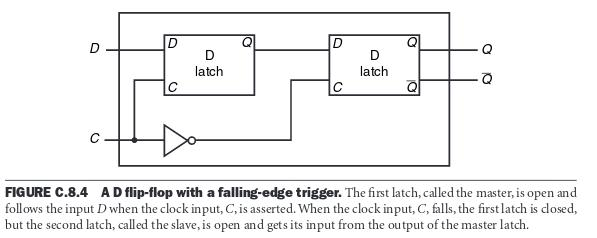
\includegraphics[scale=0.4]{flip-flop-d.jpg} 
\end{figure}
\end{frame}

\begin{frame}[fragile]
\frametitle{Diseño digital}
\begin{center}\textbf{Elementos de memoria (circuitos secuenciales)}\end{center}
\begin{itemize}
\item D Flip-Flop
el estado interno del flip-flop no cambia. Eso lo distingue de un latch.
\end{itemize}
\begin{figure}
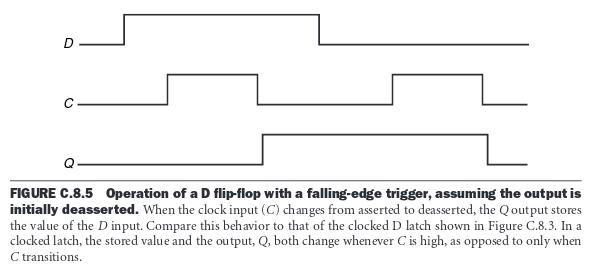
\includegraphics[scale=0.4]{flip-flop-d-tiempo.jpg} 
\end{figure}
\end{frame}

\begin{frame}[fragile]
\frametitle{Diseño digital}
\begin{center}\textbf{Elementos de memoria (circuitos secuenciales)}\end{center}
\begin{itemize}
\item D Flip-Flop
\item Si la señal D cambia cuando la señal de reloj está baja (desacertada)
el estado interno del flip-flop no cambia. Eso lo distingue de un latch.
\end{itemize}
\begin{figure}
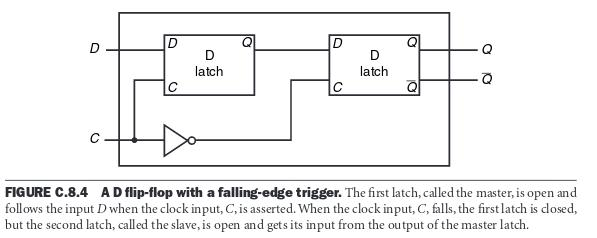
\includegraphics[scale=0.4]{flip-flop-d.jpg} 
\end{figure}
\end{frame}

\begin{frame}[fragile]
\frametitle{Diseño digital}
\begin{center}\textbf{Diseño de ALU y Registros}\end{center}
\begin{itemize}
\item Elementos de estado, multiplexores, decodificadores, ALU
\end{itemize}
\begin{figure}
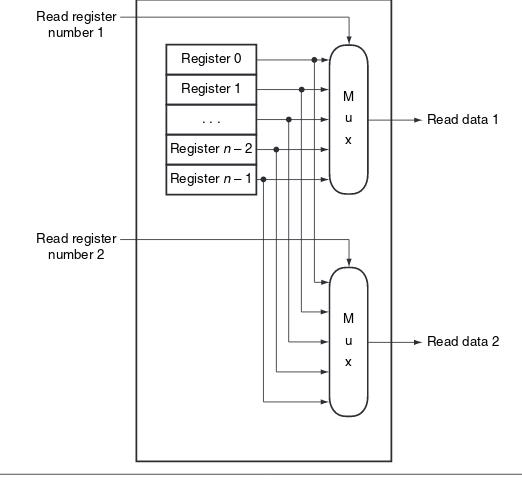
\includegraphics[scale=0.4]{leer-registro.jpg} 
\end{figure}
\end{frame}

\begin{frame}[fragile]
\frametitle{Diseño digital}
\begin{center}\textbf{Diseño de ALU y Registros}\end{center}
\begin{itemize}
\item Elementos de estado, multiplexores, decodificadores, ALU
\end{itemize}
\begin{figure}
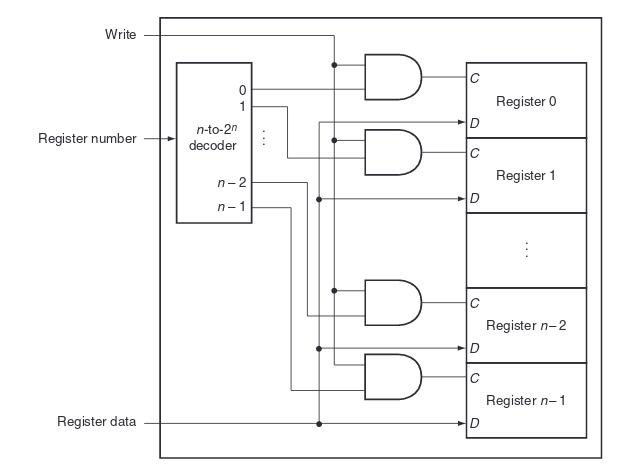
\includegraphics[scale=0.4]{escribir-registro.jpg} 
\end{figure}
\end{frame}


\begin{frame}[fragile]
\frametitle{Diseño digital}
\begin{center}\textbf{Máquinas de Estado Finito (FSM)}\end{center}
\begin{itemize}
\item Permiten especificar circuitos secuenciales
\item Ejemplo: control de la calefacción de un coche
\end{itemize}
\begin{figure}
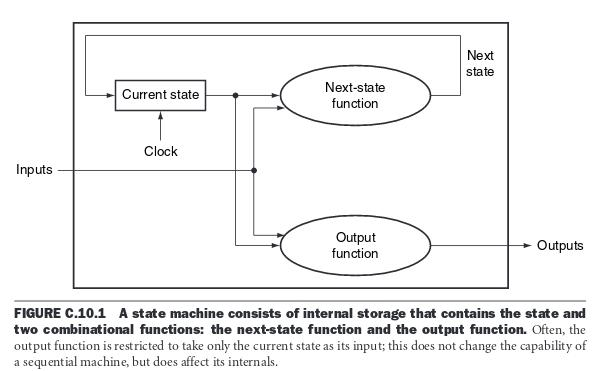
\includegraphics[scale=0.4]{fsm1.jpg} 
\end{figure}
\end{frame}


\begin{frame}[fragile]
\frametitle{Diseño digital}
\begin{center}\textbf{Máquinas de Estado Finito (FSM)}\end{center}
Existen dos clasificaciones teóricas:
\begin{itemize}
\item Autómata de Mealy
\item Autómata de Moore
\end{itemize}
\begin{figure}
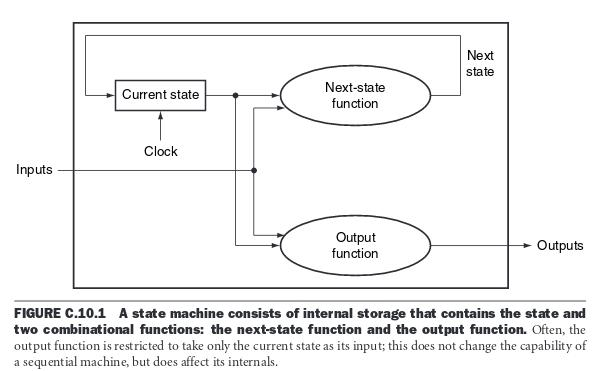
\includegraphics[scale=0.4]{fsm1.jpg} 
\end{figure}
\end{frame}



\begin{frame}[fragile]
\frametitle{Diseño digital}
\begin{center}\textbf{Máquinas de Estado Finito (FSM)}\end{center}
\begin{itemize}
\item Ejemplo: Luces de giro del Ford Thunderbird
\end{itemize}
\begin{figure}
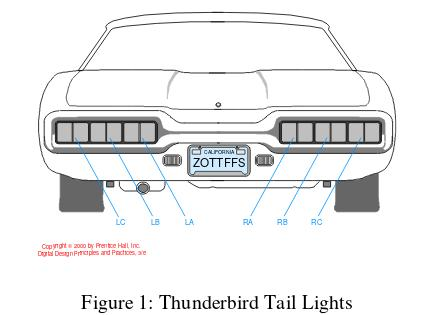
\includegraphics[scale=0.4]{fsm2.jpg} 
\end{figure}
\end{frame}

\begin{frame}[fragile]
\frametitle{Diseño digital}
\begin{center}\textbf{Máquinas de Estado Finito (FSM)}\end{center}
\begin{itemize}
\item Ejemplo: Luces de giro del Ford Thunderbird
\end{itemize}
\begin{figure}
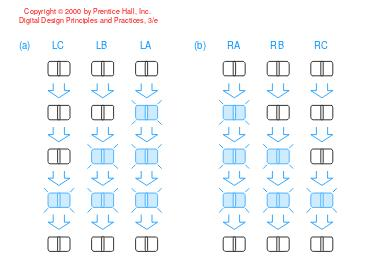
\includegraphics[scale=0.4]{fsm3.jpg} 
\end{figure}
\end{frame}

\begin{frame}[fragile]
\frametitle{Diseño digital}
\begin{center}\textbf{Máquinas de Estado Finito (FSM)}\end{center}
\begin{itemize}
\item Ejemplo: Luces de giro del Ford Thunderbird
\item Diagrama de estados
\end{itemize}
\begin{figure}
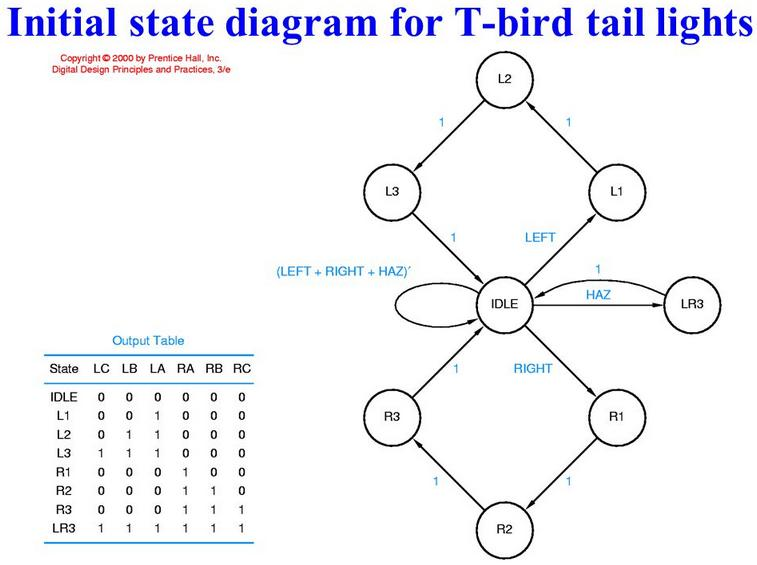
\includegraphics[scale=0.25]{fsm4.jpg} 
\end{figure}
\end{frame}

\begin{frame}[fragile]
\frametitle{Diseño digital}
\begin{center}\textbf{Máquinas de Estado Finito (FSM)}\end{center}
\begin{itemize}
\item Ejemplo: Luces de giro del Ford Thunderbird
\item Diagrama de estados (segunda versión)
\end{itemize}
\begin{figure}
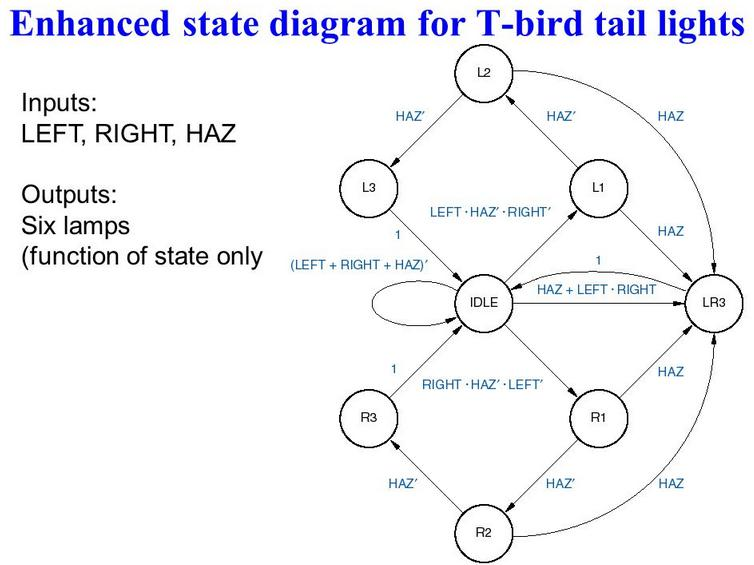
\includegraphics[scale=0.25]{fsm5.jpg} 
\end{figure}
\end{frame}


\begin{frame}
 \frametitle{Consejos y preguntas}
\begin{center}
\begin{itemize}
\item  ¿Preguntas?
\end{itemize}
\end{center}
\end{frame}


\begin{frame}
 \frametitle{Bibliografía}
Libros
\begin{itemize}
\item David. Patterson John L. Hennessy (1995), ORGANIZACIÓN Y DISEÑO DE COMPUTADORES La interfaz hardware/software, McGraw-Hill (8 copias en biblioteca).
\end{itemize}
\end{frame}


\end{document}
